%%%%%%%%%%%%%%%%%%%%%%%%%%%%%%%%%%%%%%%%%%%%%%%%%%%%%%%%%%%%%%%%%%%
%%% Documento LaTeX 																						%%%
%%%%%%%%%%%%%%%%%%%%%%%%%%%%%%%%%%%%%%%%%%%%%%%%%%%%%%%%%%%%%%%%%%%
% Título:		Apéndice A
% Autor:  	Ignacio Moreno Doblas
% Fecha:  	2014-02-01
% Versión:	0.5.0
%%%%%%%%%%%%%%%%%%%%%%%%%%%%%%%%%%%%%%%%%%%%%%%%%%%%%%%%%%%%%%%%%%%%

\pagestyle{fancy}
\fancyhead[LE,RO]{\thepage}
\fancyhead[RE]{Apéndice} %
\fancyhead[LO]{\nouppercase{\rightmark}}
%\fancyhead[RE]{Parte \thepart \rightmark} %
\chapterbegin{Proceso de integración de una aplicación node.js en Heroku}
   
   El proceso para integrar nuestra aplicación node.js en cualquiera de los servidores dedicados ofrecidos por el servicio Heroku es bastante sencillo. Asumiendo que nos hemos registrado satisfactoriamente con nuestro correo electrónico, en primer lugar debemos instalar el cinturón de herramientas Heroku, el cual puede ser accedido a través del enlace
   
   \mbox{\url{https://devcenter.heroku.com/articles/getting-started-with-nodejs}}.
    
   Este nos brinda acceso a la interfaz de comandos Heroku mediante el terminal y nos proporciona un comando local ejecutable llamado \ttw{heroku}, el cual nos ayudará a la gestión de las aplicaciones de forma local.
   La figura \ref{fig:authentication} muestra el proceso de autentificación mediante el uso del comando \ttw{heroku login}

 \begin{figure}[H] \centering
    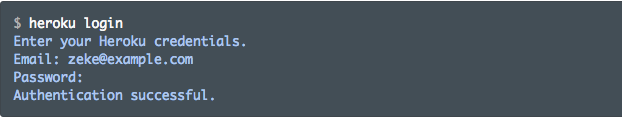
\includegraphics[width=15cm]{graphs/herokuLogin.png} \caption{Autentificación en el terminal en Heroku \cite{heroku}}\label{fig:authentication}
\end{figure}

Debemos tener en cuenta que si usamos un cortafuegos o firewall que requiere el uso de un proxy para conectarse con los servicios externos HTTP/HTTPS, tendremos que configurar las variables de entorno \ttw{HTTP\_PROXY} or \ttw{HTTPS\_PROXY} en nuestro entorno de desarrollo local previo a correr el comando.

El siguiente paso consiste en preparar la aplicación que queremos integrar en el servidor. Para ello nos situamos, localmente y desde el terminal, en el directorio el cual contiene nuestro archivo \ttw{package.json} con todas las dependencias. Debemos tener el código fuente enlazado y asociado a un repositorio git, como el proporcionado por el servicio Github por ejemplo. Ahora debemos ejecutar el comando \ttw{heroku create} para crear una aplicación en Heroku. Esto preparará a Heroku para que reciba nuestro código fuente. 

Cuando se crea la aplicación en Heroku, también se crea un repositorio remoto git llamado \ttw{heroku}, el cual estará asociado con nuestro repositorio local.

Heroku genera un nombre aleatorio para nuestra aplicación. Para asignar un nombre específico, lo pasamos como parámetro al comando. Esto se ve reflejado en la figura \ref{fig:deploy}

 \begin{figure}[H] \centering
    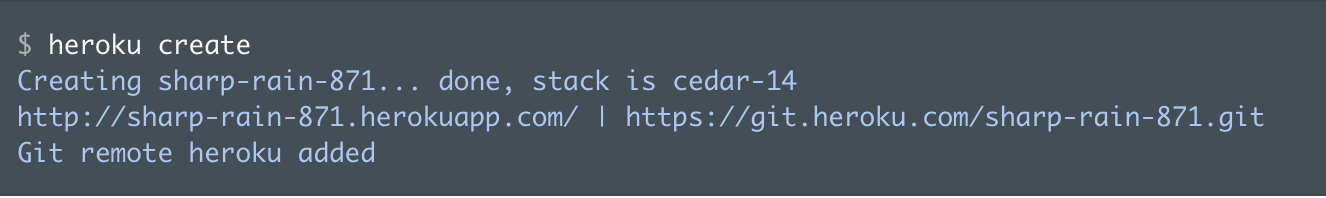
\includegraphics[width=15cm]{graphs/herokuDeploy.png} \caption{Preparando a Heroku para crear la aplicación \cite{heroku}}\label{fig:deploy}
\end{figure}

Ahora debemos enviar nuestro código fuente mediante el comando \ttw{git push heroku master}. El resultado se puede apreciar en la figura \ref{fig:push}.

 \begin{figure}[!htbp] \centering
    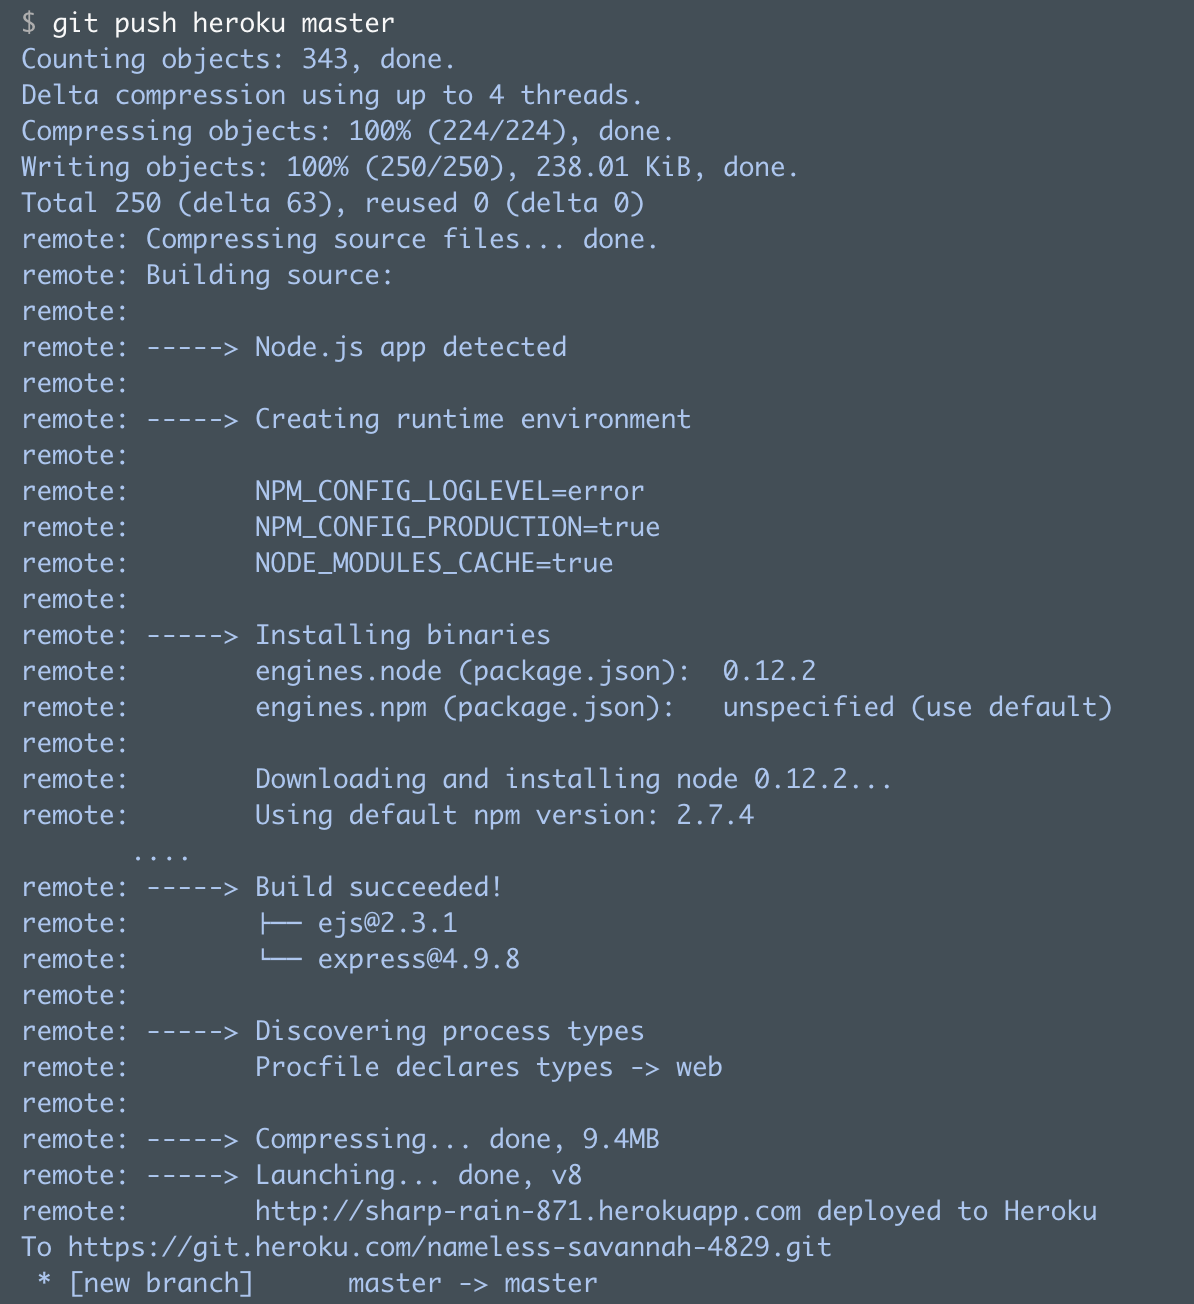
\includegraphics[width=15cm]{graphs/herokuPush.png} \caption{Enviando el código fuente a Heroku \cite{heroku}}\label{fig:push}
\end{figure}

La aplicación ya se encuentra desplegada en el servidor y podemos asegurarnos de que al menos una instancia de la aplicación está funcionando mediante el comando \ttw{heroku ps:scale web=1}.

Ahora ya podemos visitar la aplicación a través de la URL generada, en base al nombre pasado como parámetro (o el obtenido aleatoriamente). Independientemente, existe un comando útil para abrirla desde el terminal, \ttw{heroku open}.

Una vez que la aplicación se encuentra funcionando podremos consultar siempre que queramos los logs generados por Heroku y los nuestros personalizados en el código fuente a través del comando mostrado en la figura \ref{fig:logs}

 \begin{figure}[H] \centering
    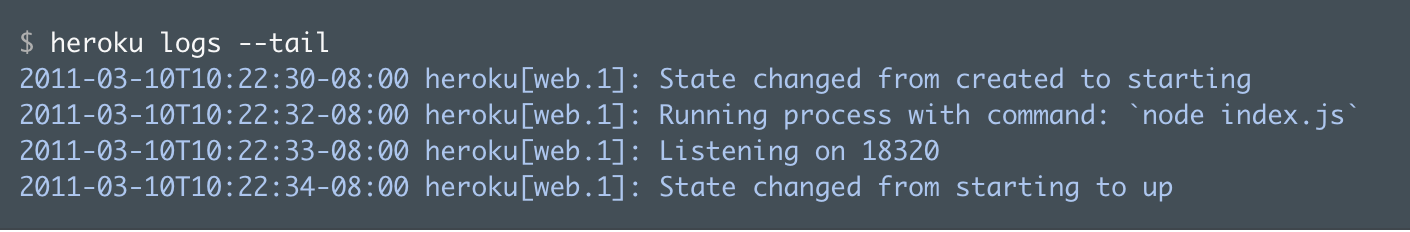
\includegraphics[width=15cm]{graphs/herokuLogs.png} \caption{Consulta de logs de nuestra aplicación \cite{heroku}}\label{fig:logs}
\end{figure}

Por último, mencionar que Heroku proporciona un Tablero de Instrumentos o Dashboard en su página web, desde el cual podremos monitorizar el estado de nuestra aplicación, controlar los permisos de acceso, configurar distintas opciones, consultar métricas específicas, etcétera. Algunas de las opciones son gratuitas y otras de pago. La interfaz presentada es la mostrada en la figura \ref{fig:dashboard}

 \begin{figure}[H] \centering
 	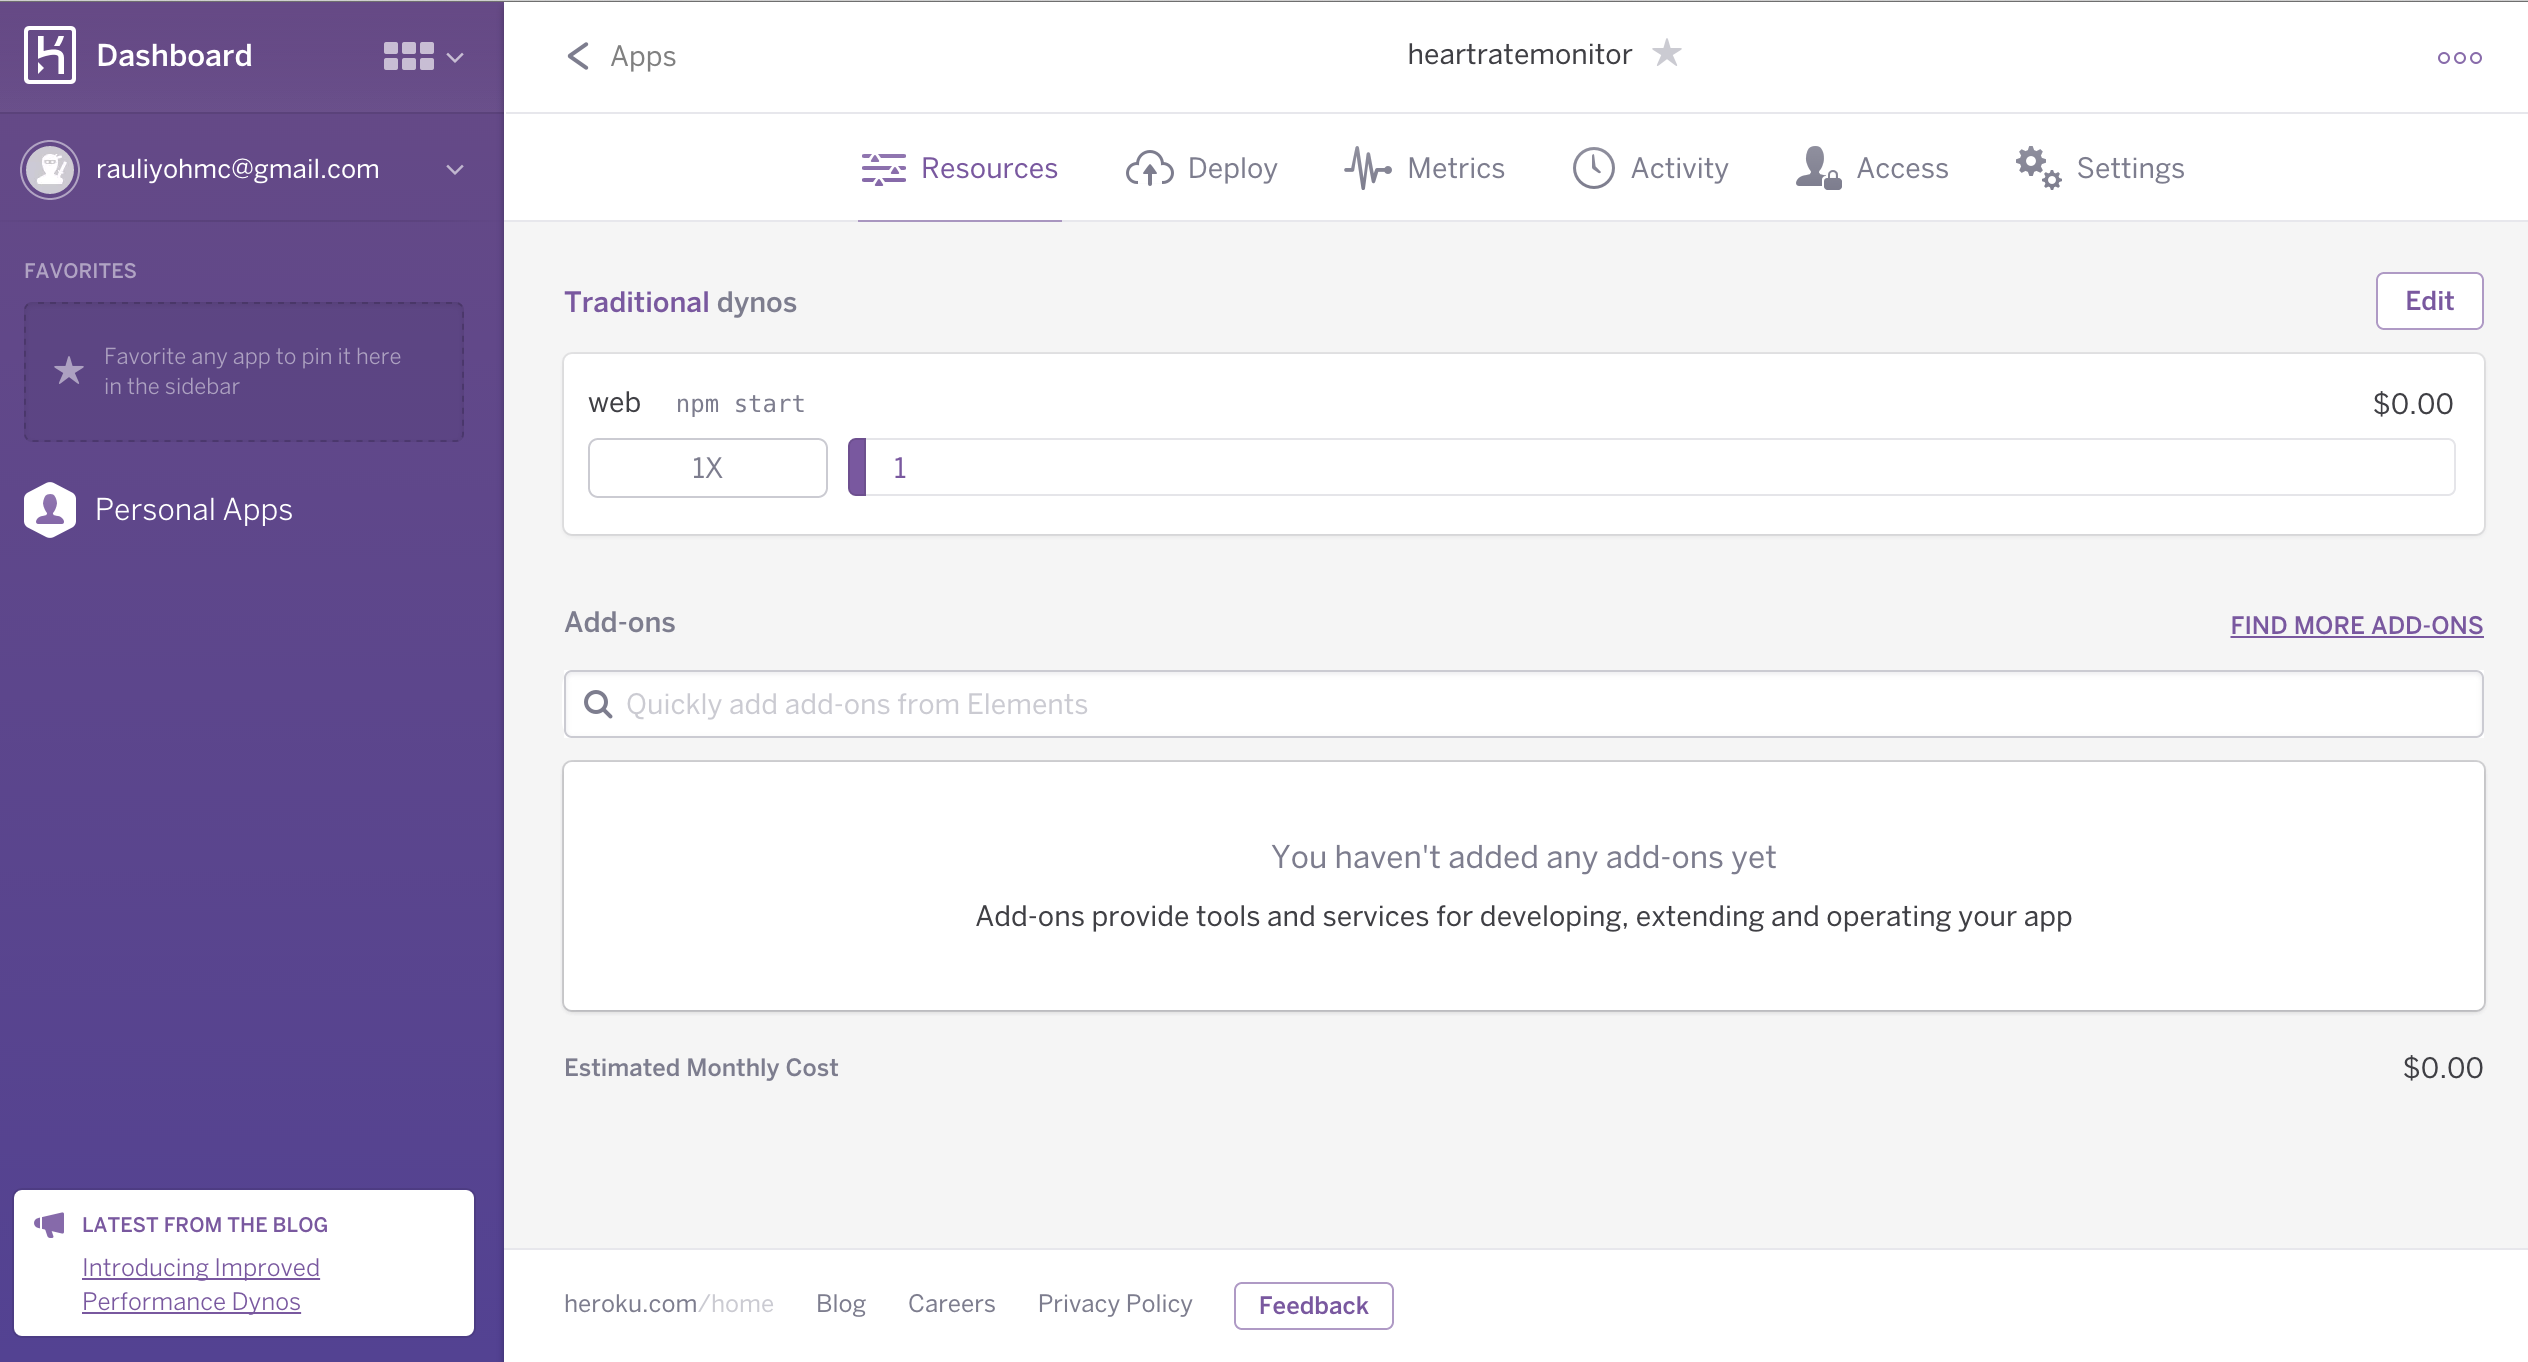
\includegraphics[width=15cm]{graphs/herokuDashboard.png} \caption{Apariencia del dashboard en Heroku \cite{heroku}}\label{fig:dashboard}
 \end{figure}

\chapterend